\chapter{CSAA的实现和数据测试}

上文中给出了CSAA的算法描述,实际实现中CSAA还采用了一些优化措施,进一步提高程序的效率。这些措施主要是从提高时间效率,空间效率
和比对准确度两个方面来考虑的。CSAA在实现时考虑到CSA查询后缀数组位置的速度较快,而由后缀数组位置查询实际的映射位置比较慢,同
时因为在做近似匹配的过程也无需具体的映射位置,所以CSAA定义了一个SAI文件,该文件是CSAA的中间输出文件,所存内容为短读序列的符合
条件的所有匹配结果,即算法\ref{alg:alignment}的返回结果组成的文件。最后通过CSAA的一个子程序结合参考序列$T$完成SAI文件到标准的
比对文件SAM文件的输出。CSAA主要包括三个子程序:build index,alignment,output。build index子程序完成对参考序列
$T$建立压缩后缀数组索引,对同一个参考序列只需建立一次索引即可。alignment子程序是CSAA的核心,完成对短读序列到参考序列$T$的映射,
输出比对的结果。最终S通过output子程序将比对结果转为标准比对结果文件SAM(Sequence Alignment/Map format)。这三个子程序的算法描述
在前文中都有所述,本章将重点讨论在实现时对效率的改进和实验测试结果。

\section{空间高效的索引算法}
本文使用的是压缩后缀数组来建立索引的,传统的构造压缩后缀数组首先需要构建后缀数组,而目前最优的后缀数组构造算法需要的内存空间
也在原文本的9倍大小,这意味着如果我们采用传统的方法建立索引,对于像人类基因组(2.8GB)这样的较大的参考序列,峰值内存将超过$25G$。
这远远超过一般PC机器的4G内存工作能力。对此我们采用文献\cite{lam2002space}提出的空间高效的压缩后缀数组构造方法作为我们的索引
构建算法。

CSAA使用的压缩后缀数组构建算法直接构建$\Phi[0\ldots n-1]$,直接跳过后缀数组的构建,总的运行时空间复杂度为$O(n(H_0+1))$位。其中
$H_0$为文本$T$的0阶经验熵,至多为$\log|\Sigma|$。而时间复杂度为$O(n\log n)$,独立于字符集大小。

设$T[0\ldots n-1]$为长为$n$的字符串序列,且$T[n-1]=\$$,令$SA_T$和$\Phi_T$为$T$的后缀数组和$\Phi$数组。假设我们已经获得了$\Phi_T$,
现在希望得到字符串$T‘ = cT$的$\Phi$数组,其中$c$为$\Sigma$的一个字符。令$SA_{T'}$和$\Phi_{T'}[0\ldots n-1]$为$T'$的后缀数组和
$\Phi$数组,首先$T'$的后缀数组是很容易从$T$的后缀数组获取的。在$T'$的所有后缀中除了$T'$本身外都是和$T$的后缀相同的,所以,$SA_{T'}$
只比$SA_T$多一个项,为获得$SA_{T'}$,我们只需要把后缀$T' _0$(下标从0开始的后缀)插入到$SA_T$中。令$x=Rank(T'_0,suffix(T))$,其
中$suffix(T)$指$T$的所有后缀,$x$即为$T'_0$在$T$的所有后缀中的字典序排名,那么据此可知后缀$T_0'$可以插入$SA_T[x-1]$和$SA_T[x]$
之间。对应的,因为在$T$最前面插了一个字符$c$,所以$SA_T$的所有数值都要加1,因为其对应的后缀的起始位置加了1。对此我们可以得出
以下引理。

\begin{lem}\label{lem:lem4}
    令$x=Rank(T'_0,suffix(T))$,那么有:
    \begin{displaymath}
        SA_{T'}[i]=\begin{cases} SA_T[i]+1 &\mbox{if } 0\leq i\leq x-1 \\
                                 0 &\mbox{if }i=x\\
                                 SA_T[i-1]+1 &\mbox{if } i\geq x+1
                    \end{cases}
    \end{displaymath}
\end{lem}

根据\ref{lem:lem4},我们可以得到以下$T$和$T'$的$\Phi$数组之间的关系。

\begin{lem}\label{lem:lem5}
    令$x=Rank(T'_0,suffix(T))$,那么有:
    \begin{itemize}
        \item $\Phi_{T'}[0]=0$
        \item 当$1\leq i <x,\Phi_{T'}[i]=\begin{cases} \Phi_T[i] &\mbox{if }\Phi_T[i]<x \\ 
                                                       \Phi_T[i]+1 &\mbox{if } \Phi_T[i]\geq x
                                         \end{cases}$
        \item 当$i=x,\Phi_{T'}[i]=\begin{cases} \Phi_T[0] &\mbox{if }\Phi_T[0]<x \\ 
                                                       \Phi_T[0]+1 &\mbox{if } \Phi_T[0]\geq x
                                         \end{cases}$
        \item 当$x<i\leq n,\Phi_{T'}[i]=\begin{cases} \Phi_T[i-1] &\mbox{if }\Phi_T[i-1]<x \\ 
                                                       \Phi_T[i-1]+1 &\mbox{if } \Phi_T[i-1]\geq x
                                         \end{cases}$
    \end{itemize}
\end{lem}

根据引理\ref{lem:lem5},我们可以提出以下的不需后缀数组,直接构建压缩后缀数组的算法。
\begin{algorithm}
    \caption{空间高效的压缩后缀数组构建算法}
    \label{alg:csaconstruct}
    \begin{algorithmic}[1]
    \Require $T,\Phi_T[0\ldots n-1],c$
    \Ensure $\Phi_{cT}[0\ldots n]$
        \State 根据$\Phi_T[0\ldots n-1]$计算字符串$T'=cT$在$T$的所有后缀中的排名$x$。
        \State 令$\Phi_{T'}[0]=x$。
        \State 对于$1\leq i\leq n$,令$\Phi_{T'}[i]=\begin{cases} \Phi_T[i] &\mbox{if } i<x\\
                                                                  \Phi_T[0] &\mbox{if } i=x\\
                                                                  \Phi_T[i-1] &\mbox{if } i>x
                                                    \end{cases}$
        \State 对于任意$1\leq i\leq n$令$\Phi_{T'}[i]=\begin{cases} \Phi_{T'}[i]+1 &\mbox{if }\Phi_{T'}[i]\leq x\\
                                                                     \Phi_{T'}[i] &\mbox{others}
                                                      \end{cases}$
    \end{algorithmic}
\end{algorithm}

按照算法\ref{alg:csaconstruct}可以递增的构建出序列$T$的$\Phi$数组,进而构建出压缩后缀数组。通过该算法建立索引所需的时间要多
于传统的构建方法,但运行时内存需求要小的多,特别是在构建像人类基因组(2.8GB)这样的大规模文本序列的索引时,有很大的优势。我们
可以在传统PC机上完成构建,无需大内存的工作站,可以节省很多成本。


\section{比对过程并行化}
CSAA给参考序列建立索引需要很多时间,但我们只需要给一个参考序列建一次索引就可以了,其后的向同一参考序列的比对无需再建立一次
索引。在比对阶段,由于一次实验的短读数量非常大,通常在几百万到数十亿条的规模,这使得比对过程通常耗时非常长。

观察比对的过程可以发现,每一条短读的比对都是独立进行的,之间互相只共享参考序列索引的数据和操作,且比对结果也是互相独立的一个
优先堆。据此,我们可以很容易的设计一个并行计算的算法来完成比对。考虑到在计算过程中需要共享参考序列索引以及匹配算法的操作。所以
CSAA选择了多线程编程模型作为并行方案。

csaa在执行比对时,可以指定线程的数量,程序启动后,将建立多个线程,并把所有的短读数据分成多份,由每个线程单独执行一份,从而实现
快速的比对。每个线程比对完成后都会把比对结果写如一个临时文件,待所有的线程执行完毕后再按顺序把比对结果输出到程序指定的文件。
具体的并行算法如算法\ref{alg:mt}所示。

\begin{algorithm}
    \caption{CSAA比对并行算法}
    \label{alg:mt}
    \begin{algorithmic}[1]
        \Require $k,\Phi,\alpha,\beta,maxPenalty,maxHeapSize$
        \Ensure $result$
        \Function{Match-MULT}{$k,\Phi,\alpha,\beta,maxPenalty,maxHeapSize$}
        \State 分割reads文件为$k$个小文件$\{read_1,read_2 \ldots read_k \}$
        \State 建立$k$个线程$threads=\{thread_1,thread_2\ldots thread_k\}$
        \ForAll{$thread_i \in thrads$ }
            \State 从文件$read_i$读取一个短读$read$
            \State \Comment{调用算法\ref{alg:alignment}}
            \State $result \gets $\Call{CSAAlignment}{$\Phi,\alpha,\beta,read,maxPenalty,maxHeapSize$} 
            \State 输出$result$到文件$result_i$
        \EndFor
        \State 合并文件$\{result_1,result_2\ldots result_k\}$到文件$result$
        \State 输出文件$result$
        \EndFunction
    \end{algorithmic}
\end{algorithm}


\section{使用seed提高比对精确度}
在DNA测序技术中,单端测序和双端测序都存在测序质量的问题。离引物结合位点越近的位置,测序结果准确率越高,而越远的位置,测序准确率
越低。根据这一现象,关于Bowtie实现的论文\cite{langmead2009ultrafast}中提出了seed的概念,概论文认为针对短读序列中测序可信度较高
的部分采用较高的限制,在较低的地方做较低的限制可以取得更精确的比对结果。如图\ref{fig:seed}所示,read前面蓝色部分是可信度
比较高的seed部分,后面是可信度比较低的非seed部分。

\begin{figure}[htbp]
    \centering
    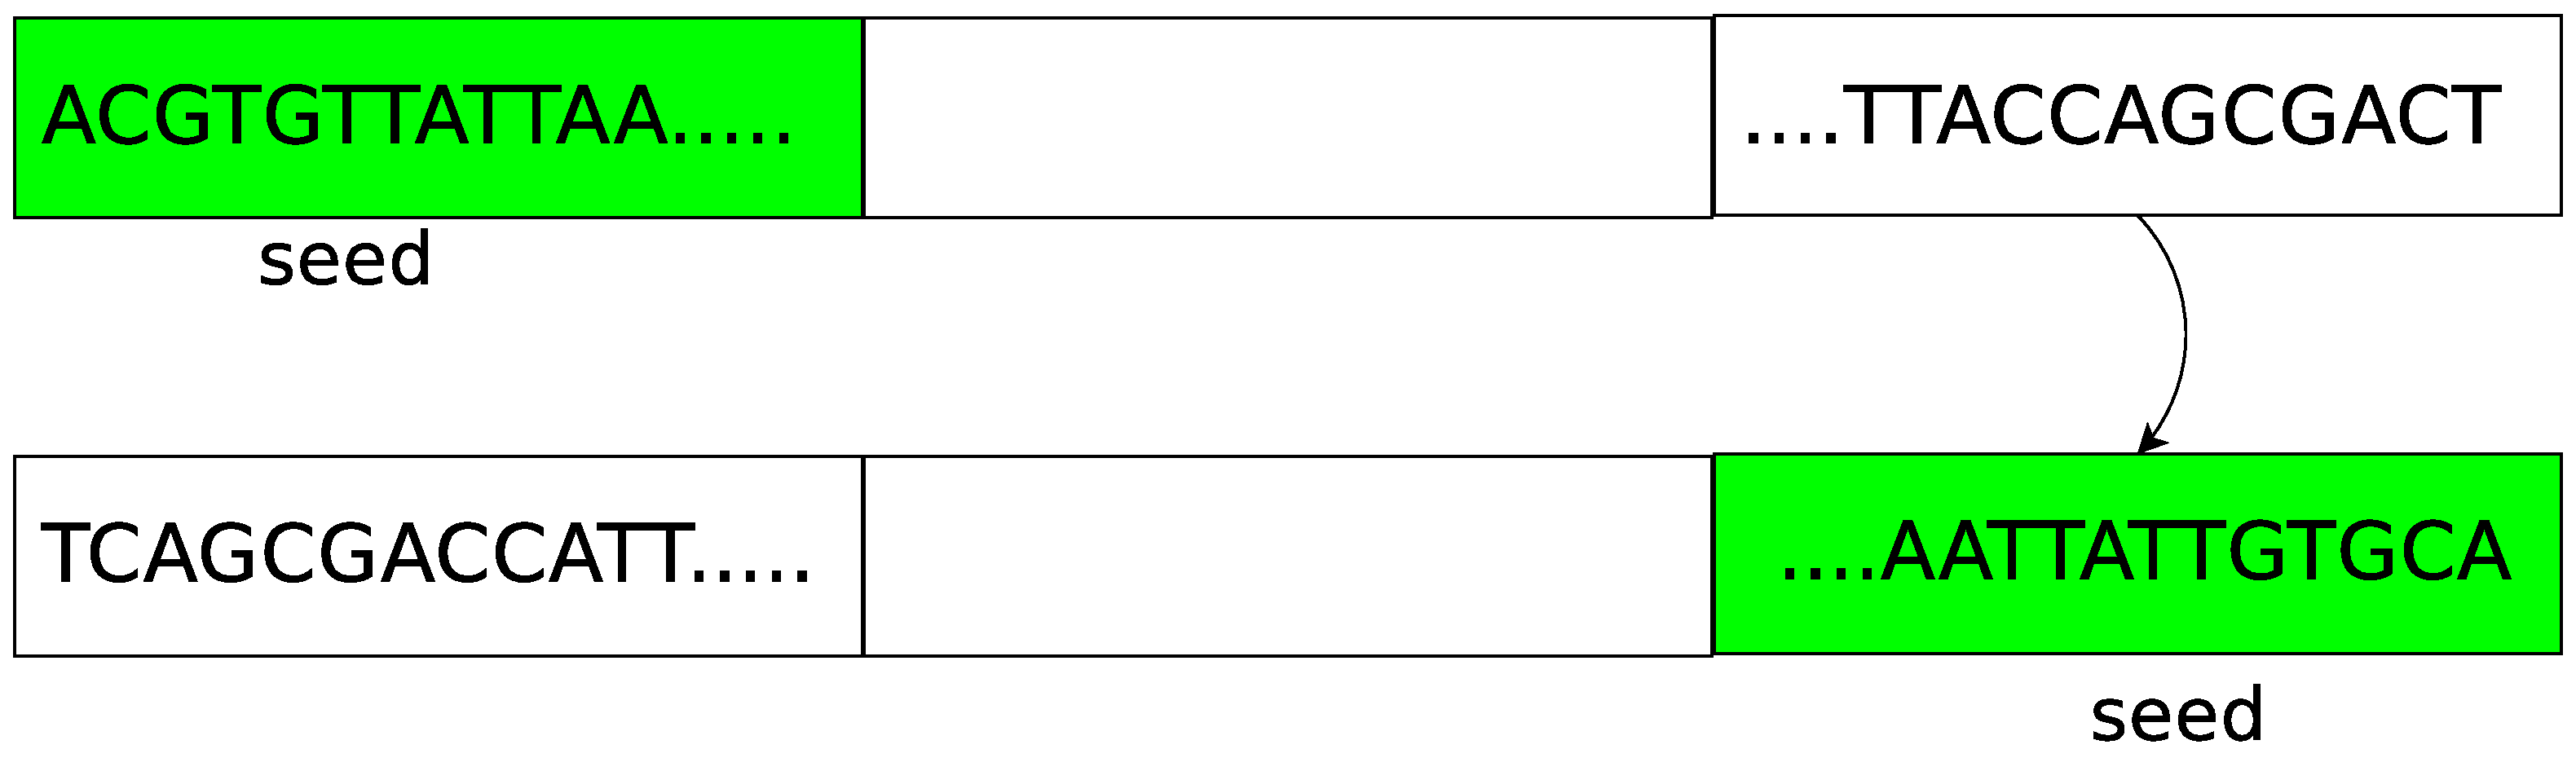
\includegraphics[width=0.7\textwidth]{seed.eps}
    \caption{seed示例} \label{fig:seed}
\end{figure}

在算法\ref{alg:alignment}中,我们当某个近似序列的$x.penalty>maxPenalty$时,会直接剪枝。CSAA中实际上是分为两部分来剪枝的,seed部有
一个$maxPenalty$,非seed部分有另一个$maxPenalty$,前者较小,后者较大。通过这样的策略,可以控制搜索结果中的待选近似序列中的替换
删除,插入等操作的绝大部分发生在非seed部分,即read的不可靠部分,从而有效提高比对的精度。至于seed的具体长度,可以根据不同的测序
技术来给定。默认情况下,Bowtie的seed长度是28,随本文发布的CSAA中seed的默认长度是32。

因为seed的限制条件较高,所以如果能首先对seed进行匹配,可以尽早抛弃掉一些不满足seed部分匹配要求,从而不用搜索非seed部分,降低空
间。但因为seed是在短读序列的前缀部分,而我们使用CSA索引的后向搜索时是从后往前搜索的,最后才搜索seed部分。所以在CSAA中无论是建
立索引还是短读匹配都是对短读的逆序序列进行的。如图\ref{fig:seed}所示,通过逆序,把read的seed部分转到后向搜索的首先搜索的部分。

\section{双端序列比对}
在前面的预备知识中我们提到了双端测序方法不同于单端测序,同一个fragement会得到两个read序列。CSAA可以支持双端数据的比对,比对的
算法和单端算法一致,分别对同一个个序列的reaed1和read2采用算法\ref{alg:alignment}进行比对,得到两个比对结果,最终使用合并程序
合并两个比对结果,得到最终比对结果。

如图\ref{fig:pairend}所示,双端测序时,因为测序精度的限制只能测序一个fragement的两端的部分数据,而大多数情况下因fragement比较
长两端的数据并不重合,所以read1和read2之间会有一个未测序的distance。。根据测序规则,序列都是从5'端开始读,因而read1和read2必然
是在DNA的不同链上,但测序时很难知道read1和read2是在DNA的某个具体链上,所以我们在比对时,需要把reaed1,read1的互补链,read2,
read2的互补连这四个序列分别和参考序列比对。但这样一来会导致需要比对四次,需要合并四个比对结果,合并的复杂度会很大。因此,CSAA
在实现时,采用了互补参考序列的方法,把参考序列和参考序列的互补序列的逆序列链接在一起,够成一个序列,从而减少了比对次数,如图
\ref{fig:merge}phase1到phase2所示。这样只需要比对两次即可,合并复杂度也降低了。

在合并read1和read2的比对结果时,CSAA除了比较两个比对结果集的比对得分之外,还通过比对distance来选定比对结果。如图\ref{fig:merge}
所示,途中phase3是一个虚拟的fragment到短读的测序示例,fragement长为10,双端测序的两个短读read1和read2都是4。通过比对程序,phase4
显示了比对的结果,可以看到,read1和read2都有两个最优的比对位置,read1的比对位置是$p1,p1'$,read2的比对位置是$p2,p2'$,由于$p2'>n$,
即该位置实在参考序列的互补链上,所以首先需要把$p2$转为参考序列的正确位置上,即$2n-p2'$,参考序列上该位置起从左向右的互补链是和
read2相匹配的。按照前文所述的双端测序方法可知,read1和read2是一个read2的两端的测序数据,所以比对的正确结果中,read1和read2的比对
位置之差应当为测序的fragement的长度,所以,双断比对的两组比对结果合并的原则即检测比对的两组比对位置的差值
是否正好是fragement的长度,符合则该比对结果是可信的比对结果,不符合则抛弃。对应的在图\ref{fig:merge}中,可以发现$p1,p2'$这一组
比对结果才是合理的,因为$|(2n-p2')-p1|$正好是phase3中的fragement的长度。

在实际测序中,我们并不能能知道fragement的准确长度,而且经过分割,复制后的fragement的长度并不是长度都相等的,只能根据测序实验方法获
取一个范围,CSAA中,默认fragement长度为200到300之间,这是illumina实验的fragement长度范围。

\begin{figure}[htbp]
    \centering
    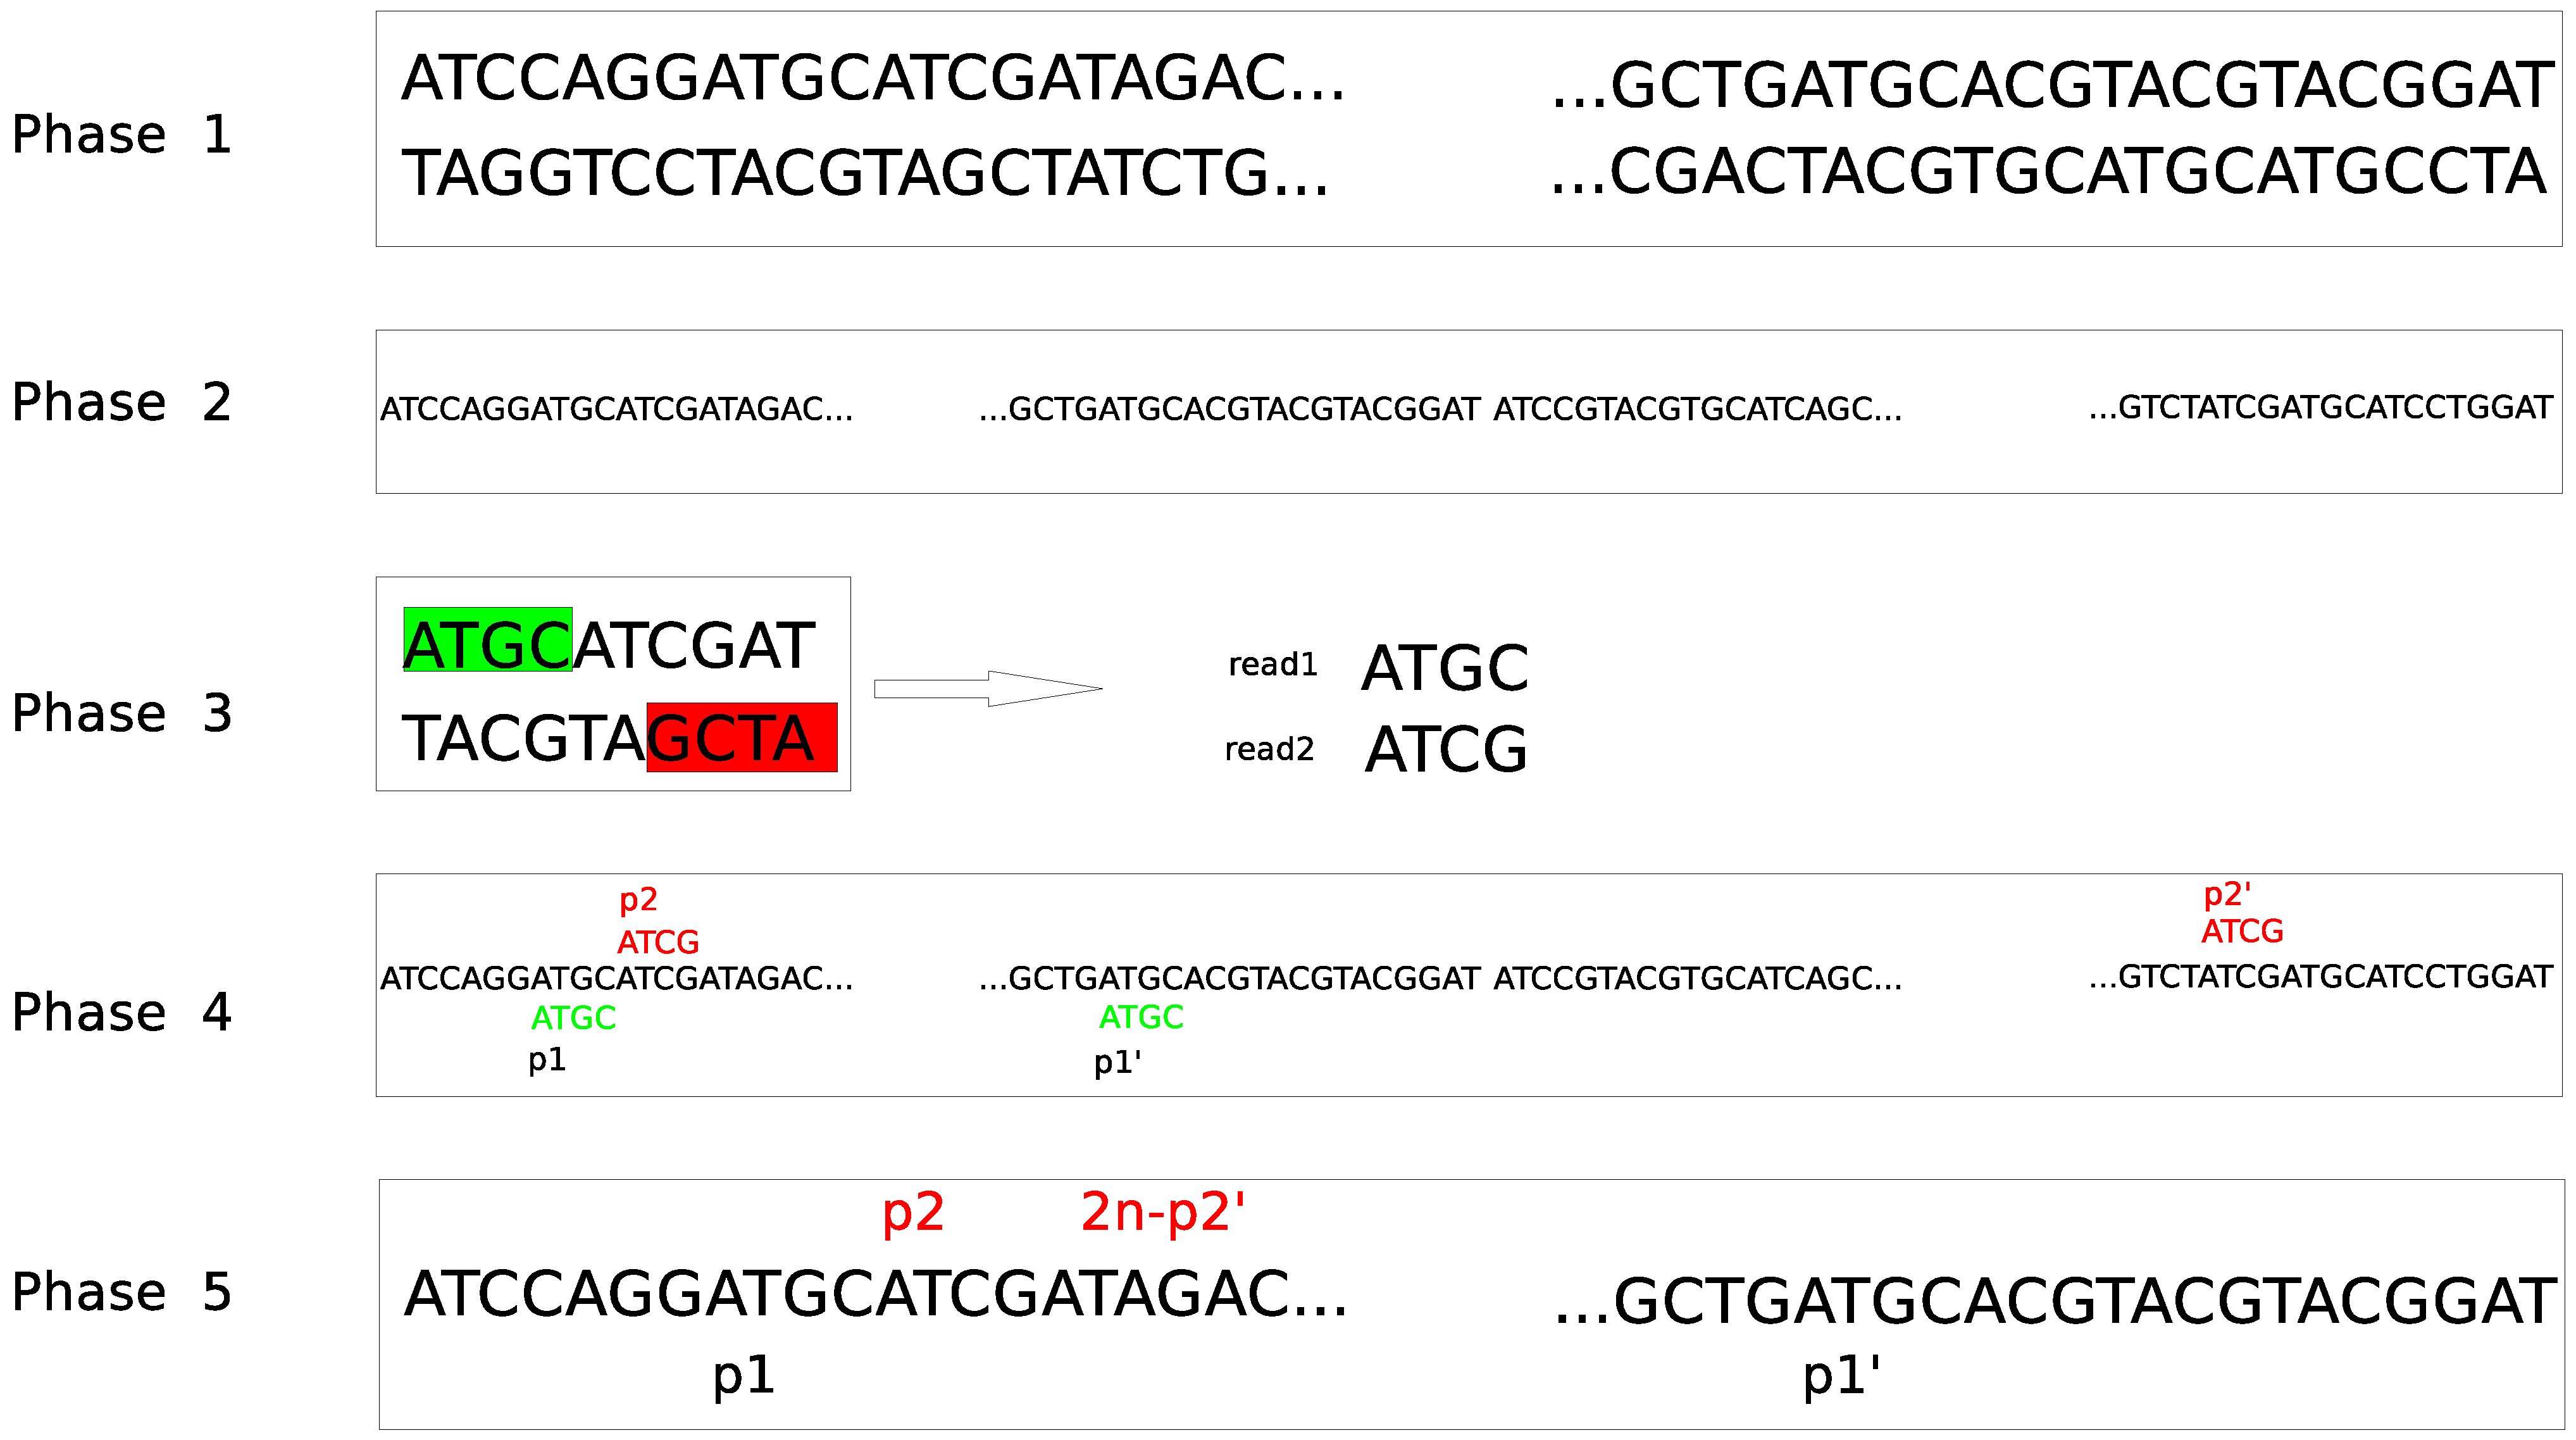
\includegraphics[width=0.95\textwidth]{merge.eps}
    \caption{双端比对示例} \label{fig:merge}
\end{figure}


\section{CSAA对比实验测试}

为测试CSAA的性能,本文同时测试了MAQ\cite{li2008mapping},Bowtie\cite{langmead2009ultrafast}和BWA\cite{li2009fast}这三个比对工
具,和CSAA进行比较。分别对比这几个工具在不通规模数据上建立索引时的时间,需要的内存;以及在模拟数据上和真实数据上的比对能力。
MAQ为所有的短读序列建立hash表,进而遍历整个参考序列来实现比对。Bowtie和BWA是用基于BWT的索引建立
的比对工具,其中Bowtie采用了回溯法实现替换操作,但不支持insert和delete操作,即上文中所论述的gap alignment。BWA除了支持insert,
delete之外,还加入了smith-water方法提高比对精度。比对测试中,我们的csaa和bwa,bowtie等都只使用单线程运行。

\subsection{测试环境和数据}

在对CSAA的对比测试中,我们使用gcc 4.6.3编译链接,并且使用了-O3优化。系统环境为ubuntu 12.04 amd64,运行在一台具有18G内存的工
作站上。测试使用的数据是标准的人类基因组序列hg18.fa,来自1000 Genome Project的NCBI build 36,模拟数据也是在该数据上生成。所
有测试数据均使用默认选项运行。

\subsection{索引建立时间}
表\ref{tab:tab1}中对比了bowtie,BWA和CSAA三种工具分别建立索引时所需要的时间和内存消耗对比情况,表中数据分别对应几个工具在索引
512M,1024M和2048M的数据时所需要的时间和内存。测试使用的各个数据均来自NCBI build 36数据的截取数据。

\begin{table}[htbp]
    \caption{建立索引的时间空间对比}
    \label{tab:tab1}
    \centering
    \begin{tabular}{lrrrrrr}
        \hline
        \multirow{2}{*}{Program} & \multicolumn{3}{c}{Time(s)} & \multicolumn{3}{c}{Memory(M)}\\
        \cline{2-4}
        \cline{5-7}
        & 512M &1024M &2048M &512M &1024M &2048M\\
        \hline
        Bowtie&1311 &2720 &5581 &987 &1109 &1210 \\
        BWA&531 &1101 &2445 &1890 &1902 &2006 \\
        CSAA&413 &843 &2065 &2483 &5325 &11435 \\
        \hline
    \end{tabular}
\end{table}

从表\ref{tab:tab1}中的测试结果可以看到,CSAA相对其他两个不对工具在索引时间上具有较大优势,这是由于BWA和Bowtie都同时给inverted
reference建立了索引,用时会较长。其中Bowtie建立索引时是分块建立索引的,最终再合并成一个索引,时间效率最差,但需用内存空间最小。

\subsection{模拟数据测试}
本文使用SAMtools工具包中的wgsim工具从人类基因组序列中随机生成模拟的短读序列。然后,分别用四种比对工具对这些模拟的short
短读s序列进行比对,然后测试比对结果。因为这些模拟数据在参考序列上的映射位置是已知的,所以就可以计算出各个工具的比对结果的
精确率。

表\ref{tab:tab2}所示为四个测试工具的比对结果展示,参考序列是人类基因组序列,模拟短读序列的长度为70bp,总共有1000000个
短读,所有序列均为single end序列。

\begin{table}[htbp]
    \caption{模拟数据比对测试}
    \label{tab:tab2}
    \centering
    \begin{tabular}{lrrrr}
       \hline \\
       Program&Time(s)&Memory(M)&Conf(\%)&Err(\%)\\
       \hline \\
       Bowtie&1701&2911&86.3&0.2\\
       BWA&1519&3116&90.7&0.12\\
       CSAA&2241&2905&89.9&0.13\\
       \hline
    \end{tabular}
\end{table}

表\ref{tab:tab2}中的实验的模拟数据使用wsgi程序在人类基因组上生成的长为70bp,生成过程中,单核苷酸变异(SNP)的概率是0.09\%,
indel变异的概率是0.01\%,indel的长度是满足正太分布$N(500,50)$。
对比结果中conf是有确定的比对结果的短读的比率,指的是所有短读中比对程序可以比对到映射位置的短读所占比例。
而Err错误率是指在所有的有确定映射位置的短读中的比对位置错误的短读的比率。从中可以看出,在长为70bp的100万个短读的映射中,CSAA相
对于BWA和Bowtie在查询时更节省内存,在确定率和错误率上和BWA持平,优于Bowtie。出现这样的结果是因为BWA和CSAA都支持indel操作,而
Bowtie则只支持substitution操作,当短读序列比较长时其比对效果就会下降。

\subsection{真实数据测试}
为测试CSAA在真实数据上的表现,本文从网络上下载了12.2 million个长为51bp的短读数据。这些数据来自European Read Archive(AC:ERR000589)
,是1000 Genomes Project的一个名男性基因组测序,由Illumina测序技术完成测序。参考序列选的是人类基因组,测序编号NCBI build 36。

\begin{table}[htbp]
    \caption{实际数据比对测试}
    \label{tab:tab3}
    \centering
    \begin{tabular}{lrrr}
       \hline \\
       Program&Time(m)&Memory(M)&Conf(\%)\\
       \hline \\
       Bowtie&303&3122&84.6\\
       BWA&221&3887&88.4\\
       CSAA&409&3313&86.5\\
       \hline
    \end{tabular}
\end{table}

表\ref{tab:tab3}中的测试结果显示,在实际数据中CSAA也具有较高的准确性,86\%的短读序列都能映射到参考序列上,
基本性能和BWA接近,相对BWA使用更少的内存空间。

\section{本章小节}

本章主要介绍了CSAA在实现方面所做的一些优化,以及相应的优化的实验效果展示。本章首先在第一节介绍了改进后的压缩后缀数组索引算法
在空间方面的效率。第二节主要介绍采用并行化方法提高比对效率的方法和效果。第三节介绍seed的概念以及采用seed提高比对精确度的方法。
第四小节紧接着描述了CSAA对双端测序的支持。最后一小节通过综合比对测试,对比CSAA和常见的几种比对程序的比对效果,可以看到CSAA在
比对精度和时间上还是有很大的优势的。
